\documentclass[../main.tex]{subfiles}
\begin{document}
\chapter{Reduce and Conquer}
\label{chapter_divide_conquer}
\begin{chapquote}
{Albert Einstein, }
``Everything should be made as simple as possible, but not simpler.''
\end{chapquote}

This chapter is the essence of the algorithmic problem solving--`Reduction'. 


\begin{importantnote}
Reduction is the essence of problem solving, and self-reduction is the ``center'' of the essence. Recurrence relation is our tool from math. The correctness of self-reduction is proved with mathematical induction. And the complexity analysis relies on solving recurrence relation. 
\end{importantnote}


\section{Introduction}
\paragraph{Story}Imagine that your mom asks you to get 10,000 pounds of corns, what would you do? First, you would think, where should I get the corns? I can go to Walmart or I can go to grow the corns in the farm. This is when one problem/task is reduced to some other problems/tasks. Solving the other ones means you solved your assignment from your mom. This is one example of the reduction; converting  problem  $A$ to problem $B$.

Now, you are at Walmart and are ready to load the 10,000 pounds of bagged corns, but the trunk of your car can not fit all corns at once. You just decide that you want to do 10 rounds of loading and transporting to home. Now, your task becomes loading 1,000 pounds of corns. After you are done with this, you just solved a subtask--getting 1,000 pounds of corns. In the second round, you load another 1,000 pounds. You solved another subtask--getting 2,000 pounds of corns. After 10 rounds in total, you will solve the original task. This is the other side of reduction, reduce one problem to one or multiple smaller instances of itself. 


\paragraph{Definition of Reduction} In computational theory and computational complexity theory, a reduction is an algorithm for transforming one problem $A$ into another problem or other problems. There are two types of reduction:
\begin{enumerate}

    \item \textbf{Self-Reduction}: it can also be a problem that are just a smaller instance or we say \textit{subproblems} of itself, say if the original problem is $a_n$, then the smaller problems can be $a_{n/2}$, $a_{n-1}$, $a_{n-2}$, and so on. Self-reduction is a recursive process; we reduce the problem into one or more subproblems of smaller size recursively until the subproblem is small enough to be a base case. We need to differentiate whether the subproblem is reduced by constant factor or just by constant size.
\begin{itemize}
    \item If it is by constant size,  say $a_{n-k}$, this will characterize \textit{searching},  \textit{dynamic programming} and \textit{greedy algorithm}. 
    \item If it is by constant factor,  say in the form of $a_{n/b}$, b is integer $b\geq 2$, this can be used to characterize  \textit{divide and conquer} which we detail on it further in Section.~\ref{sec_divide_conquer}.

\end{itemize}
 The \textbf{Recurrence relations} which we have put so much effort on in last chapter will conveniently represent and interpret the relation  between problem and its subproblems in self-reduction. Optionally, we can also use \textit{recursion tree} to help with visualization. In the next two sections, we shall see how and discuss additional techniques for each type. 
    \item \textbf{$A$ to $B$}: The other problem can be a totally different problem, say $B$. Intuitively, if we know how to solve $B$, this induces a solution to $A$. On the other hand, this also means that if any of $A$ and $B$ is unsolvable, then it indicates or proves that the other is unsolvable. More details will be given in Section.~\ref{chapter_reduce_conquer_sec_a_b}.
\end{enumerate}

\subsubsection{Reducing a Problem to Subproblem(s)} ``Reducing'' a problem into subproblem(s) as the first step of using self-reduction will result potentially two types of subproblems: \textit{non-overlapping subproblems} and \textit{overlapping subproblems}. 

\paragraph{Non-overlapping subproblems} Like cutting a rod into multiple pieces, the resulting  subproblems each stand alone, disjoint with each other and become another rod which is just smaller. The most general way is to divide equally,  thus conventionally $a_{n/b}$ means the problem is reduced into non-overlapping subproblems and each with size $n/b$. 

\paragraph{Overlapping subproblems} Different from the non-overlapping problems, the feature of overlapping problem is more abstract. Easily put, it means subproblems share subproblems. Say $a_n$ is reduced to $a_{n-1}$ and $a_{n-2}$, and according to this recursive rule, $a_{n-1}$ will be reduced to $a_{n-2}$ and $a_{n-3}$. Now we can see that problem $a_n$ and $a_{n-1}$ both share a common subproblem $a_{n-2}$, this is to say that these problems might overlap. Overlapping subproblems is one of the signals that further optimization might apply, which is detailed in Dynamic programming in Chapter.~\ref{chapter_dynamic-programming}.


\subsubsection{Self-Reduction and Mathematical Induction}
The word `self-Reduction' is not commonly or even put under the umbrella of `reduction'. In other materials, you might see that the content of self-reduction appears in the form of mathematical induction\footnote{Such as \textit{Introduction to Algorithms: A Creative Approach}.}. Self-Reduction and Mathematical Induction  are  inseparable, as self-reduction can be represented with recurrence relation, and the mathematical induction is the most straightforward and powerful tool to  prove its correctness and their concentration aligns--``concentrating on reducing a problem and solving subproblems  rather than solving it directly''.

Mathematical induction can guide us to reduce the problem: we assume we know the solution from problems of size $a_{n/b}$, or $a_{n-k}$, we focus on how to construct a solution for $a_n$ with solutions to our subproblems such as $a_{n/b}$ and $a_{n-k}$. 
 
We will further see the distinction of these two characteristics of problems in our following examples.



%%%%%%%%%%%%%%%%%%%%%%%%Divide and conquer%%%%%%%%%%%%%%%%%%%%%%%
\section{Divide and Conquer}
\subsection{Concepts}
\label{sec_divide_conquer}
\begin{figure}[h]
    \centering
    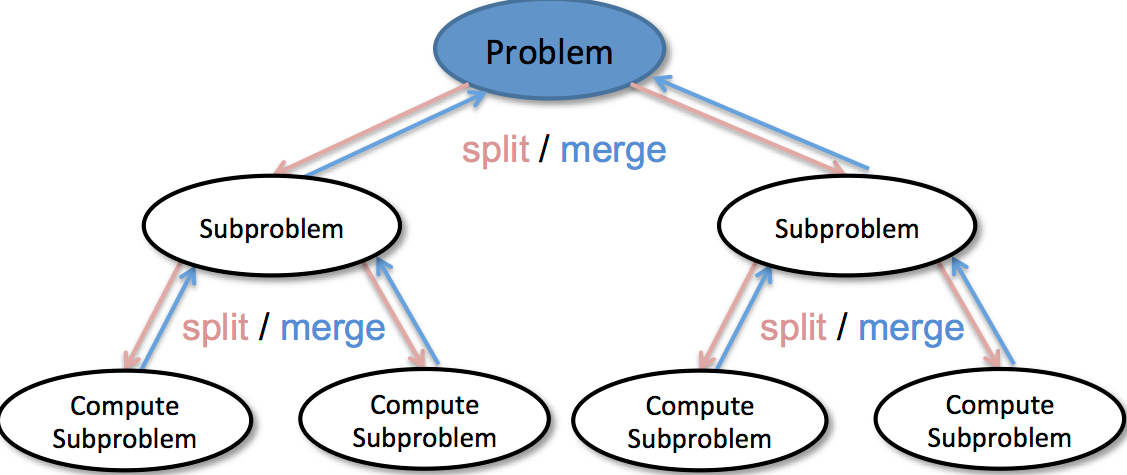
\includegraphics[width=0.8\columnwidth]{fig/divide_conquer.png}
    \caption{Divide and Conquer Diagram}
    \label{fig:divide_conquer}
\end{figure}
Divide and conquer is the most fundamental problem solving paradigm for computer programming; the strategy is to divide a problem into smaller problems recursively until the subproblem is trivial to solve. In more details, it consists of two process:
\begin{enumerate}
    \item \textbf{Divide:} divide one problems into a series of non-overlapping subproblems that are smaller instances of the same problem recursively until reaching to the \textit{bases cases},  when the subproblem is trivial to solve. Usually, the problem is divided equally, and most likely breaking into half and half. We say a problem of size $n$, denote as $p_n$ is divided into $a$ subproblems and each with size $n/b$, denote as $a p_{n/b}$, $a, b$ are mostly integer and $a\geq 1, b\geq 2$. As we explained in Chapter.~\ref{chapter_iteration_recursion}, this process happens at the top-down pass. 
    \item \textbf{Conquer:} this step means that in the bottom-up pass, say we have the solutions of the $a$ subproblems each with size $n/b$ available, we need to \textit{combine} these solutions to our  current problem of size $n$.
\end{enumerate}
We can interpret the divide and conquer  with a recurrence relation as in Eq.~\ref{divide_conquer_relation}
    \begin{equation}
        p_n= \Psi(n,a p_{n/b})
        \label{divide_conquer_relation}
    \end{equation}
    $\Psi$ will no longer be a function any more, but instead it represents the operations needed to combine the the solutions to subproblems to solution of current problem, $n$ means the size of the combined solutions will be mostly $n$, which also means $n$ elements. 

\paragraph{Decrease and Conquer}
When $a=1$,  each problem reduced to only one sub-problem, and this case is named as \textbf{Decrease and Conquer}. Decrease and conquer will reduce search space each step. If our time complexity is $T(n) = T(n/2)+O(1)$, we get $O(\log n)$. This decrease and conquer method cuts the search space into half of its original at each step until it reaches its target. Because logarithmic is way faster even compared with linear, this is a significant efficiency growth. We will discuss classical algorithms with this paradigm such as Binary Search, Binary Search Tree, Segment Tree in the next chapter. 
\subsubsection{Common  Applications of Divide and Conquer}
 Divide-and-conquer is mostly used in some well-developed algorithms and some data structures. In this book, we covered the follows:
\begin{itemize}
    \item Various sorting algorithms like Merge Sort, Quick Sort (Chapter~\ref{chapter_sorting});
    \item Binary Search (Section~\ref{sec_binary_search});
    \item Heap(Section~\ref{sec_heap});
    \item Binary Search Tree (Section~\ref{sec_binary_search_tree});
    \item Segment Tree(Section~\ref{sec_segment_tree}).
\end{itemize}
    
% We can further represent its time complexity with recurrence relation:
% \begin{equation} \label{dp_equation}
% \begin{split}
% T(n) &= T(n-1) + T(n-2) +...+T(1) + f(n)\\
% \end{split}
% \end{equation}
    
\subsection{Hands-on Examples}
\subsubsection{Merge Sort}
The concept can be quite  dry, let us look at a simple example of merge sort. Given an array, [2, 5,1,8,9], the task is to sort the array to [1, 2, 5, 8, 9]. To apply divide and conquer, we first divide it into two halves: [2, 5, 1], [8, 9], sort each half and with return result [1, 2, 5], [8, 9], and now we just need to merge the two parts. The process can be represented as the following:
\begin{lstlisting}[language=Python]
def divide_conquer(A, s, e):
    # base case, can not be divided farther
    if s == e:
        return A[s]
    # divide into n/2, n/2 from middle position
    m = (s+e) // 2

    # conquer 
    s1 = divide_conquer(A, s, m)
    s2 = divide_conquer(A, m+1, e)
    
    # combine
    return combine(s1, s2)
\end{lstlisting}
\begin{figure}[h!]
    \centering

    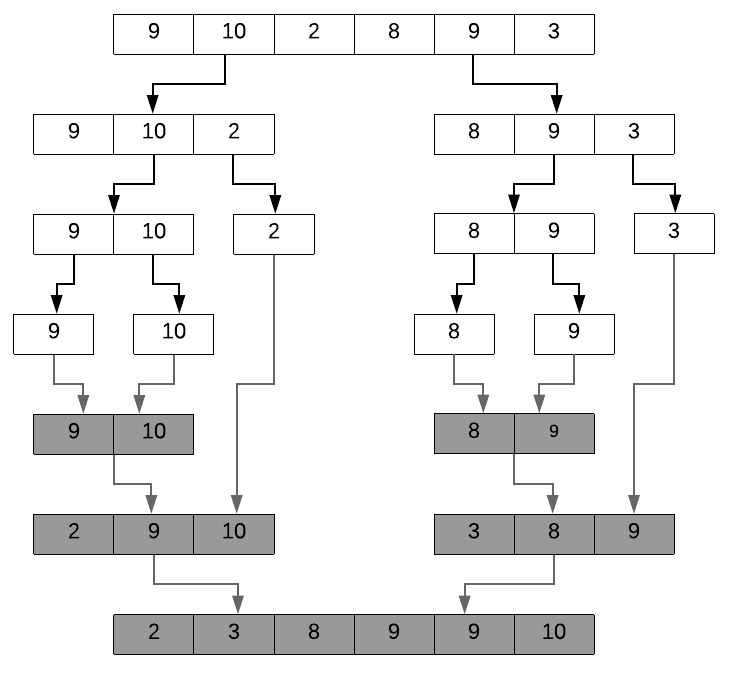
\includegraphics[width=0.9\columnwidth]{fig/merge_sort.png}
    \caption{Merge Sort with non-overlapping subproblems where subproblems form a tree}
    \label{fig:merge_sort_tree}
\end{figure}
This process can be visualized in Fig.~\ref{fig:merge_sort_tree}. From the visualization, we can clearly see that all subproblems form a tree and they never interact or overlap with each other, and each subproblem will only be visited once.

\subsubsection{Maximum Subarray (53. medium).}
Find the contiguous subarray within an array (containing at least one number) which has the largest sum.
\begin{lstlisting}[numbers=none]
For example, given the array [-2,1,-3,4,-1,2,1,-5,4],
 the contiguous subarray [4,-1,2,1] has the largest sum = 6.
\end{lstlisting}
\textbf{Solution: divide and conquer.} $T(n) = max(T(left),T(right), T(cross))$, max is for merging and the T(cross) is for the case that the potential subarray across the mid point. For the complexity, $T(n)=2T(n/2)+n$, if we use the master method, it would give us $O(nlgn)$. We write the following Python code
\begin{lstlisting}[language = Python]
def maxSubArray(self, nums):
        """
        :type nums: List[int]
        :rtype: int
        """
        def getCrossMax(low,mid,high):
            left_sum,right_sum =0,0
            left_max,  right_max = -maxint, -maxint
            left_i,right_j=-1,-1
            for i in xrange(mid,low-1,-1): #[)
                left_sum+=nums[i]
                if left_sum>left_max:
                    left_max= left_sum
                    left_i = i
            for j in xrange(mid+1,high+1):
                right_sum+=nums[j]
                if right_sum>right_max:
                    right_max= right_sum
                    right_j = j
            return (left_i,right_j,left_max+right_max)
        
        def maxSubarray(low,high):
            if low==high:
                return (low,high, nums[low])
            mid = (low+high)//2
            rslt=[]
            #left_low, left_high, left_sum = maxSubarray(low,mid) #[low,mid]
            rslt.append(maxSubarray(low,mid)) #[low,mid]
            #right_low,right_high,right_sum = maxSubarray(mid+1,high)#[mid+1,high]
            rslt.append(maxSubarray(mid+1,high))
            #cross_low,cross_high,cross_sum = getCrossMax(low, mid, high)
            rslt.append(getCrossMax(low, mid, high))
            return max(rslt, key=lambda x: x[2])
        return maxSubarray(0,len(nums)-1)[2]
\end{lstlisting}





%%%%%%%%%%%%%%%%%%%%%%%%%%%Reduction by constant size%%%%%%%%%%%%%%%%%%%%%%%%%%%%%%
\section{Constant Reduction}
\label{chapter_reduce_conquer_constant_size}
\subsection{Concepts}
In this category, problem instance of size $n$ is reduced to one or more instances of size $n-1$ or less recursively until the subproblem is small and trivial to solve. This process can be interpreted with Eq.~\ref{dp_relation_by_constant_size}.
    \begin{equation}
    p_n = \Psi(n, p_{n-1}, p_{n-2}, ..., p_{n-k})  \text{ for $n \leq k$,}
    \label{dp_relation_by_constant_size}
    \end{equation}
The number of subproblems that a current problem relies on should be as less as possible. The ideal option is when it only relates to  $n-1$, this is the case of an exhaustive search, which can be implemented easily both with recursion and iteration. 

\subsubsection{Overlapping Subproblems} When the number of the subproblems appears in this relation is larger or equals to 2, the subproblems might overlap. This implies that a straightforward recursion based solution without optimization will be expensive because these overlapped problems are solved again and again; the optimization is possible with dynamic programming or greedy algorithm shown in Part.~\ref{part_dp_greedy} which optimize it using \textit{caching mechanism} by saving the solution of each subproblem and thus avoiding recomputation. However, to stick to just the reduction itself, we delay our examples' possible optimization to Part.~\ref{part_dp_greedy}.

\subsubsection{Subproblem Space} To count all possible subproblems-- the subproblem space--is important for us to understand the complexity. For array, a subproblem can be a subarray that $[a_i,...,a_j], i<j, i\in[0,n-1], j\in[0,n-1]$, which makes the potential subproblems $n^2$. Sometimes, it is enough to fix $a_i=a_0$, that the subarray always start from the start. The reduction by constant size will be less likely to be seen in tree structure where its more organized by the divide and conquer reduction. In graph, this type of reduction??? In practice, we shall always try to define our subproblems that comes with smallest possible surbproblem space, we would only enlarge it when we feel the further shrinking will make the construction of the solution impossible. 

\subsection{Hands-on Examples}
\paragraph{Example 2: Fibonacci Sequence}
\begin{figure}[h!]
    \centering
    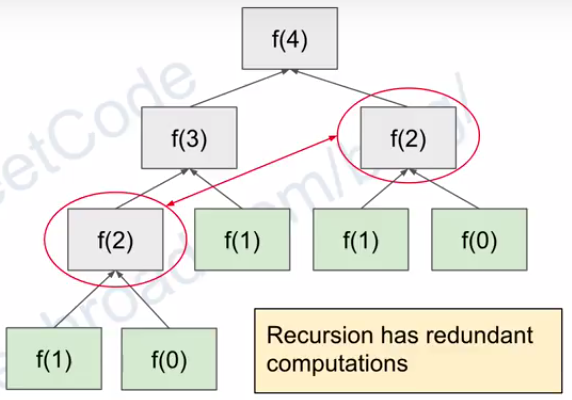
\includegraphics[width=0.6\columnwidth]{fig/fibanacci.png}
    \caption{Fibonacci number with overlapping subproblems where subproblems form a graph.}
\label{fig:fibonacci_overlap}
\end{figure}
The Fibonacci Sequence is defined as:
\begin{lstlisting}[numbers=none]
Given f(0)=0, f(1)= 1, f(n) = f(n-1) + f(n-2), n>=2. Return the value for any given n.
\end{lstlisting}
The above is the classical Fibonacci Sequence, to get the fibonacci number at position n, we first need to know the answer for subproblems f(n-1) and f(n-2), we can solve it easily using recursion function:
\begin{lstlisting}[language=Python]
def fib(n):
    if n <= 1:
        return n
    return fib(n-1) + fib(n-2)
\end{lstlisting}
The above recursion function has recursion tree shown in Fig~\ref{fig:fibonacci_number}. And we also draw the recursion tree of recursion function call for merge sort and shown in Fig~\ref{fig:merge_sort_tree}. We notice that we call f(2) multiple times for fibonacci but in the merge sort, each call is unique and wont be called more than once. The recurrence function of merge sort is $T(n) = 2*T(n/2)+n$, and for fibonacci sequence it is $T(n) = T(n-1)+T(n-2)+1$. 

\paragraph{Maximum Subarray} Using reduction by constant size, the problem is to find a subarray $a_i,a_{i+1}, ...,a_{j}, i>=0, i\geq j<n$. Now, let's assume that the solution of subarray of size $n-1$ is known with the induction hypothesis, try to figure out the ``operations'' to construct the solution for $n$.

For subproblem of size $4$, it is [-2,1,-3], where is the maximum subarray? A naive and human doable way is to check all subarries, which will be
\begin{lstlisting}[numbers=none]
subarray start from -2: -2, -1, -4
subarray start from 1: 1, -2
subarray start from -3: -3
\end{lstlisting}
we would find $[1]$ is our maximum subarray, to subproblem [-2,1,-3,4], to construct the solution, we have two cases:
\begin{enumerate}
    \item $j=n-1$, to put 4 inside, we just need to make a choice in three cases: previous maximum subarray $[a_i,...,a_{n-1}$, extented maximum subarray $[a_i,...,a_{n-},a_{n}$, and $[a_n]$.
    \item $j\neq n-1$, in this case, say our maximum subarray is $[a_i,...,a_j], j\neq n-1$, the ecase of extension is more complex, that we need to try extend any item in $[a_{j+1},a_n]$. Its doable but gives us time complexity of $T(n)=T(n-1)+O(n)$, this is the same as of in the naive solution to enumerate all subarries. 
\end{enumerate}
%%%%%%%%%%%%%%%Summary section
 \section{Divide-and-conquer VS Constant Reduction} Therefore, we draw the conclusion: 
 \begin{enumerate}
     \item For non-overlapping  as Eq.~\ref{divide_conquer_eq}, when we use recursive programming to solve the problem directly, we get the best time complexity since there is no overlap between subproblems.
     \item For overlapping problems as Eq.~\ref{dp_equation}, programming them recursively would end up with redundancy in time complexity because some subproblems are computed more than one time. This also means they can be further optimized: either using recursive with memoization or iterative through tablization as we later explain in Chapter \textbf{Dynamic Programming} (Chapter~\ref{chapter_dynamic-programming}. 
 \end{enumerate}
 \paragraph{Practical Guideline}
With the master theorem to either divide and conquer or reducing by constant size tells us its asympototic time complexity: divide and conquer is either polynomial or logarithmic and reducing by constant size will go up to exponential with $f(n)\geq n$. This reminds us that when our problem state space is beyond exponential, we might better try reducing by constant size, and if the problem state space is within polynomial, a divide and conquer should work better to further boost the efficiency. 
 
 %%%%%%%%%%%%%%%%%%%%%%%%%%%%A to B%%%%%%%%%%%%%%%%%%%%%%%%%%%%%%%%
\section{A to B}
\label{chapter_reduce_conquer_sec_a_b}
\subsection{Concepts}
\paragraph{Definition}
Reduction or transformation between two problems $A$ and $B$ is to say that a solution of one problem is also a solution of the other. It's common applications are:
\begin{enumerate}
    \item Design algorithms: given algorithm for $B$, can solve our problem for $A$.
    \item Proving limits: If A is hard that its lower bound is known, then so is B.
    \item Classifying problems using the established relative difficulty of problems.
\end{enumerate}
The strategy is to reduce problem $A$ into a more general-purposed problem. One of such general-purposed problem is \textit{linear programming}, which we study in Chapter.~\ref{}. Only experience and study of the classical algorithms designed on a certain data structures can help us identify possible `patterns'. In this section, we emphasize the principle of this method instead of pointing out all possible reduction; as we are further in the book and the journey of practice, we will learn.


\subsection{Practical Guideline and Examples}
\paragraph{Sorting and Ordering is always a good try.}
We only focus on Design algorithms in this book with this method. In practice, \textit{sorting} or \textit{ordering} is a common trick to reduce a problem to another that is more structured and with well-known algorithms to solve.  For example, if we need to find the k-th largest item in an array, sorting the array first serves a more general purpose and solves the problem. Same with the problem that we are given an unsorted array, find if there exist duplicate items. This case fully demonstrated how a well-known and a general purposed sorting algorithm can be used to solve a problem that might seems bizarre or unique. 

However, more likely sorting will be a subroutine of our algorithm design, whose purpose is to order our input in the hope that it simplifies the following design. Similar examples can be found across the book, other example will be in the convex hull problem where the points are sorted by angle to outskirt chosen point. The real-world is fuzzy, as a computer scientist, we are responsible to enforce orders, so always keep this in mind. 

\paragraph{Other Reduction Examples}

There are also more creative reduction,  as we see in the last section of example maximum subarray, we were having a problem to use straightforward induction hypothesis, we can strengthen our hypothesis.

If we reduce our problem to be: find the maximum subarray that ends at $n$, that is find $[a_i,...,a_{n-1}], i>=0$ in the array that has the maximum value. We simply only have $n$ candidates to compare. To constrcut this reduced problem B back to A, the maximum subarray of A is the maximum subarray of $n$ problems of B, say $[a_0]$, $[a_0, a_1]$, ..., $[a_0,...,a_{n-1}]$. The rule of reduction can happen into B, that is case $j=n-1$ in the original problem is enough to construct it. We can write $p_n=\max(p_{n-1}, p_{n-1}+a_n, a_n)$. 

In the array, a \textit{suffix} is defined as any subarry which includes its last item. Another way to put the induction hypothesis into the problem B: We know how to find the maximum suffix of size $k<n$, we can easily induce the maximum suffix of size $k+1$.

Another more creative option we convert this problem to best time to buy and sell stock problem.[0, -2, -1, -4, 0, -1, 1, 2, -3, 1], => O(n), then we use prefix\_sum, the difference is we set prefix\_sum to 0 when it is smaller than 0, O(n)
\begin{lstlisting}[language = Python]
from   sys import maxint
class Solution(object):    
    def maxSubArray(self, nums):
        """
        :type nums: List[int]
        :rtype: int
        """
        max_so_far = -maxint - 1
        prefix_sum= 0
        for i in range(0, len(nums)):
            prefix_sum+= nums[i]
            if (max_so_far < prefix_sum):
                max_so_far = prefix_sum
 
            if prefix_sum< 0:
                prefix_sum= 0  
        return max_so_far
\end{lstlisting}
% We know if the array is empty, then the empty array is our target with 0 as its maximum sum. For any non-empty array, what is the possible solution? It can be zero is all items in the array are negative, otherwise it must be a subarray that has a non-negative sum with at least one item. From another angel, the problem equals to a problem that find the maximum value between the maximum subarray for $n$ subsequences that ends at each index--suffixs. For example, in this case, it becomes find the maximum value of the following problems:













 
 






\section{The Skyline Problem}
Define and solve it by two cases.

Both skyline problem and maximum subarray problem has illustrated how we can use reduction to solve our problem, either self-reduction or the $A$ to $B$ is used. The real algorithm design is usually a  composite of multiple design steps and methods. 
 
% %%%%%%%%%%%%%%%%%%%%%%%%%%%%%%%%%%%%%%%%%%%%%%%%%%%%%%%%%%%%%%%%%%%%%%%%%%%%%%%%%%%%%
% %%%%%%%%%%%%% Recursive Programming
% %%%%%%%%%%%%%%%%%%%%%%%%%%%%%%%%%%%%%%%%%%%%%%%%%%%%%%%%%%%%%%%%%%%%%%%%%%%%%%%%%%%%%%%%%
% \section{Recursive Programming}
% For recursive function, we can draw recursive tree to denote the state transfer graph. With recursive function, it can simplify the programming of certain programs, once we mastered recursive function, we would feel it is a lot simpler than iterative implementation. However, it does take extra space complexity compared with the iterative implementation. 

% \paragraph{Recursion}

% \paragraph{Recurrence Function} For recusrive program, we need to figure out the recursive transfer function between $f(i)$ and the next level $f(i+1)$. For example, the fibonacci number we could have $f(i) = f(i-1) + f(i-2)$. For the merge sort, we cant use a math function to represent this operation, we have $T(n) = 2*T(n/2) + O(n)$. $f(i) = merge(f(left), f(right))$. Some recursive function would have redundancy which we can improve the efficiency and avoid to compute the same subproblem twice by memoization which saves the result, and the iterative peer of the recursive implementation is called \textit{dynamic programming}. We will discuss the dynamic programming in details in the following chapter ~\ref{dynamic-programming}. Some other recursive function, there is no overlaps between subproblems which are the \textit{divide and conquer} cases, which will be discussed in detain in chapter~\ref{divide-conquer}. Or we have the universal \textit{Depth-first-searching} which can be implemented with recursive function, we will include this in chapter~\ref{searching}. 

% % \textbf{Recursive Function and Tree Structure}: 



% % 递归函数关注以下几个因素
% % ·退出条件
% % ·参数有哪些
% % ·返回值是什么
% % ·局部变量有哪些
% % ·全局变量有哪些
% % ·何时输出
% % ·会不会导致堆栈溢出
 


%%%%%%%%%%%%%%%%%%%%%%%%%%%%%%%%%%%%%%%%%%%%%%%%%%%%%%%%%%%%%%%%%%%%%%%%%%%%%%%%%%%%%
%%%%%%%%%%%%% Exercises
%%%%%%%%%%%%%%%%%%%%%%%%%%%%%%%%%%%%%%%%%%%%%%%%%%%%%%%%%%%%%%%%%%%%%%%%%%%%%%%%%%%%%%%%%
\section{Exercises}
\begin{enumerate}
    \item Binary Search.
    \item Use Self-Reduction by constant size to solve maximum subarray problem. 
    \item Skyline problem.
\end{enumerate}

\end{document}